\begin{solutionbox}{\stretch{-1}}\newline
\section*{1. Plot of $f(xrcfgvfr) = \frac{x^2 + 2x + 1}{x^2 + 3x +3}$}
\[
    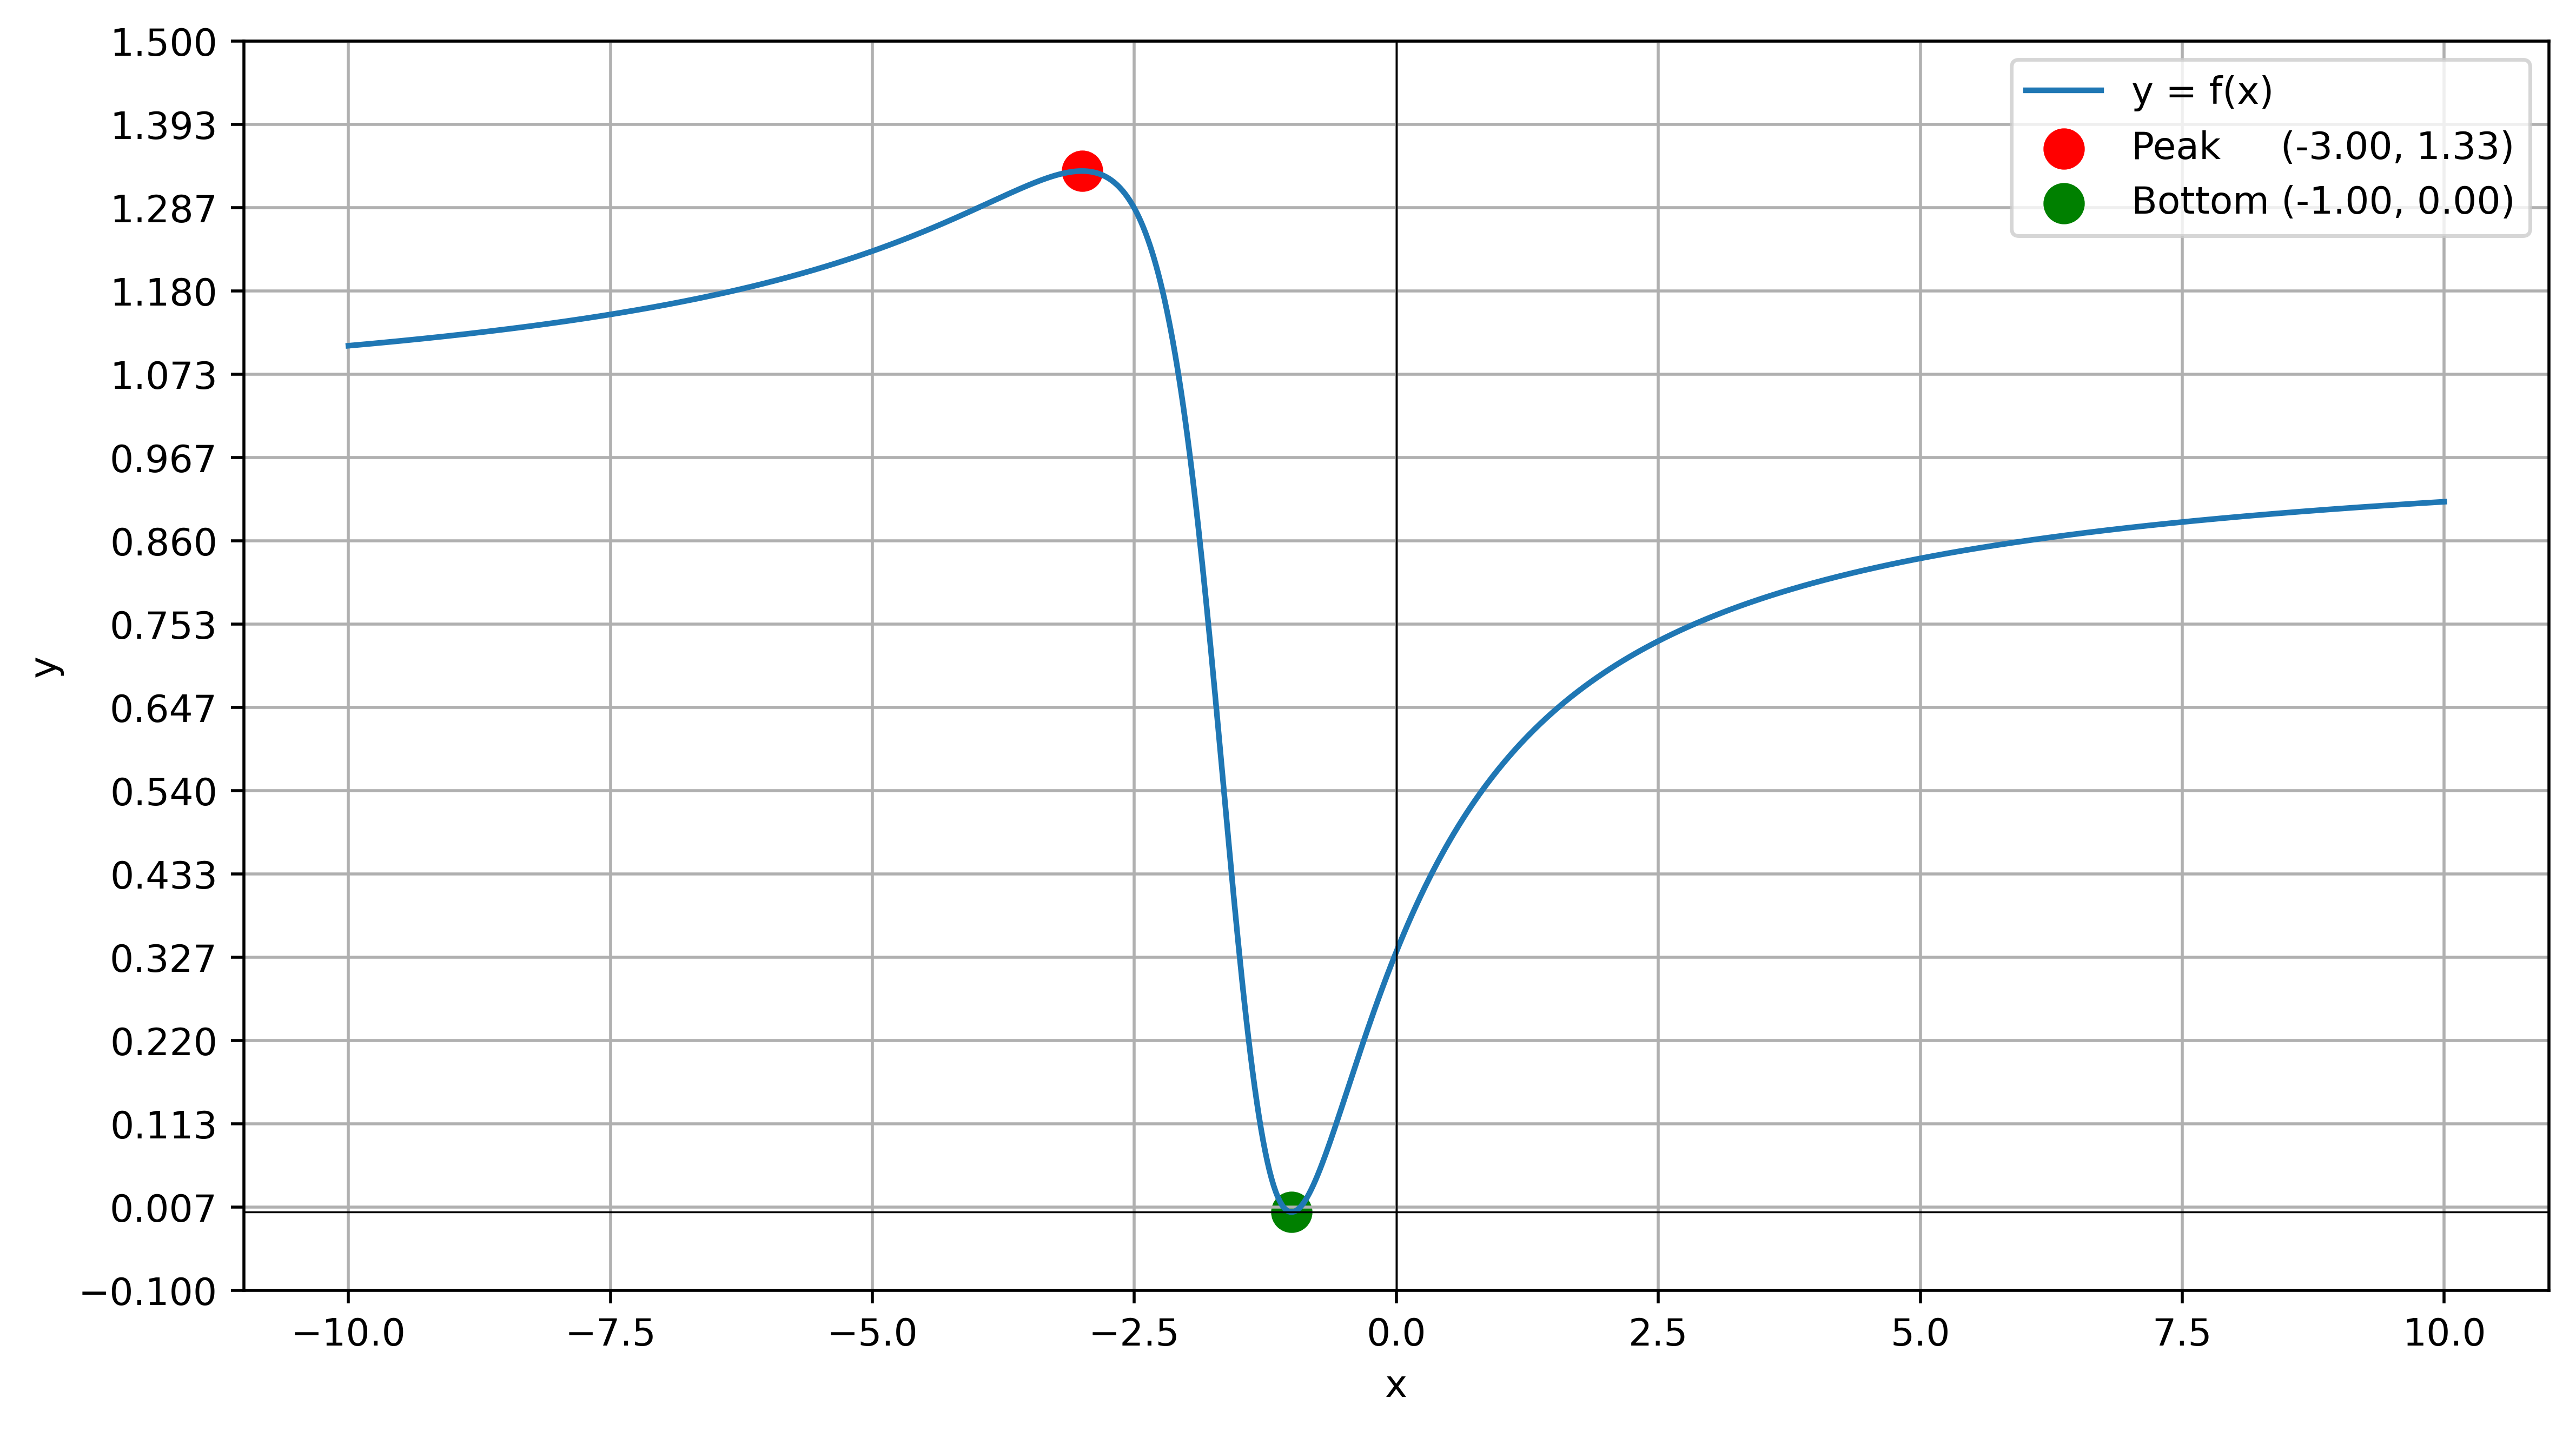
\includegraphics[scale=0.7]{plot.png}
\]

\end{solutionbox}
\newpage
\begin{solutionbox}{\stretch{-1}}\newline

\section*{2.}
\[
    f(x) = \frac{g(x)}{h(x)}= \frac{x^2 + 2x + 1}{x^2 + 3x + 3}
\]

\[
    f'(x) = \frac{(f'(x)g(x))+(f(x)g'(x))}{(g(x))^2}
\]

\[
    = \frac{(2x+2)(x^2 + 3x + 3) - (x^2 + 2x + 1)(2x+3)}{(x^2 + 3x + 3)^2}
\]

\[
    = \frac{(2x^3 + 6x^2 + 6x + 2x^2 + 6x + 6)-(2x^3 + 3x^2 + 4x^2 + 6x + 2x + 7)}{(x^4+3x^3 + 3x^2 + 3x^3 + 9x^2 + 9x + 3x^2 + 9x + 9)}
\]

\[
    = \frac{(2x^3 + 8x^2 + 12x + 6 - 2x^3 - 7x^2 - 8x - 3)}{(x^4 + 6x^3 + 15x^3 + 18x + 9)}
\]

\[
    = \frac{x^2 - 4x + 3}{x^4 + 6x^3 + 15x^2 + 18x + 9}
\]

\[
    = \frac{(x+1)(x+3)}{(x^2 + 3x + 3)^2}
\]

\subsection*{Critical Points:}

\[x = -1\]

\[x = -3\]

\section*{3.}
The formula for $f'(x)$ is:
\[
 f'(x)= \frac{(x+1)(x+3)}{(x^2 + 3x + 3)^2}
\]

See section 2. for full proof.
\end{solutionbox}
\newpage
\begin{solutionbox}{\stretch{-1}}\newline


\section*{4.}

% TODO: DO THIS AND DO THAT!

\end{solutionbox}
